\chapter{Conclusion}
\label{chapter:conclusion}

%\minitoc
\chapterwithfigures{\nameref*{chapter:conclusion}}
\chapterwithtables{\nameref*{chapter:introduction}}

\ifthenelse{\boolean{skipConclusion}}{\endinput}{}

This thesis primarely focuses on the \ac{NVS} problem, especially in the the highly constrained single-view scenario. In this chapter, we briefly review our core contributions before outlining the current landscape in \ac{AI} and 3D. The final section of this manuscript is devoted to the perspectives and potential further work that may stem from this PhD thesis.  

\section{Summary}

This manuscript has adressed, to a large extent, the single-image \ac{NVS} problem. Our first two contributions were built around deep learning architectures that synthesize a novel viewpoint of static scenes from single source posed images. Our latest contribution has a primary industrial aim, where novel views are rendered from a scene explicitly reconstructed in 3D as a gaussian point cloud.

We began this manuscript by presenting our epiponarNVS architecture in Chapter \ref{chapter:epipolarnvs}. Our main motivation for this work was to propose an innovative way to encode camera pose information for an image-to-image \ac{CNN} in single-view \ac{NVS}. While most prior work often discretized \citep{kim2020novel} or encoded camera pose information into a low dimensional signal \citep{sun2018multiview}, we instead exploited the epipolar constraint to encode such prior information. Through a vanilla grid sampling strategy on the source view, we get colored epipolar lines that we stored as an image, fed alongside the source image to pose-condition the neural network. 

In Chapter \ref{chapter:epinerf}, we investigated how epipolar constraints could be integrated into a generalizable \ac{NeRF} architecture for single-image \ac{NVS}. Based on a \textit{source-aligned} dense feature volume produced from a \ac{CNN}-encoder, we trained a novel \ac{NeRF}-architecture, termed NeRFeature, to produce \textit{target-aligned} features. These \textit{source} and \textit{target-aligned} feature are ultimately used through an epipolar constraint in a light attention mechanism. We extensively shown in the Experiments section \ref{subsec:epinerf/experiments} how our multi-stage training architecture might help generalizable \ac{NeRF} to better perfrom on single-image \ac{NVS} tasks.  

Chapter \ref{chapter:gausssplat} was finally devoted to the \ac{NVS} solution we began investigated with CarCutter - Meero.  While research and open-source projects around \ac{GS} \citep{kerbl20233d} are tremendously prolific and progressing steadily or more than a year now \citep{luiten2023dynamic,yang2024gaussianobject,wewer24latentsplat}, we presented several improvements to extend beyond the original 3D \ac{GS} work. A denser point cloud using the visual hull concept was introduced at the initialization stage, gaussians opacity was made view-dependant through an additional \ac{MLP}, allowing for better rendering of transparent surfaces, and a novel denfification strategy was implemented. However, 3D \ac{GS}-based scenes remain prone to artifacts, as discussed in \ref{sec:gs-limitation}, especially when rendered at non-training locations. Further development will therefore focus on improving novel view synthesis at these \textit{out-of-distribution} locations. The introduction of geometric priors and constraints during training (such as depth loss and normals surface regularization) is also curently under development. 

In addition to these contributions, we introduced AdaptativeSR in Appendix \ref{chapter:appendix}, an approach that considers topological issues in single-image 3D reconstruction. This module aims to refine the topology of a genus-0 mesh by relying solely on 2D silhouette masks and the differentiable renderer from \citep{liu2019soft}. While this contribution is more closely related to 3D reconstruction than \ac{NVS}, this work, as Chapter \ref{chapter:gausssplat}, creates a meaningful connection between the two concepts. 

\section{Perspectives and further work}
We present in this section few perspectives and suggest further research directions that could be explored following this PhD thesis. We have made every effort to draw parallels and connections between current 3D \ac{AI} research and industry. 

\subsection{Further work}
This thesis tried to integrate and leverage on geometric priors and constraints whithin deep neural architectures devoted to \ac{NVS} and 3D reconstruction. When we first began exploring epipolar considerations years ago, few works has attempted to do so. \ac{NVS} was initially addressed through an image-to-image \ac{CNN}, disregarding the physical image formation process and its inherant 3D/2D projection. Our second contribution moves closer to the 3D domain by developing a feature epipolar-based attention mechanism within a generalizable \ac{NeRF} architecture. Our lastest work around 3D\ac{GS} bridges the gap between 3D reconstruction and \ac{NVS} since the learned 3D gaussian cloud is used as an intermediate representation to render novel views at stabilized locations. We present below a few directions and specific topics in these areas that could be addressed in future work.

\noindent \textbf{Single-image 3D reconstruction.} 3D \ac{AI} research is currently extremely prolific when it comes to addressing single-image 3D reconstruction (and thus inherently \ac{NVS}). Within the last 12 months, at least three powerful and solid project has been released:  One-2-3-45++ \citep{liu2023one2345++} in November 2023 ,TripoSR \citep{tochilkin2024triposr} in March 2024 and InstantMesh \citep{xu2024instantmesh} in April 2024. The fomers two were outperformed by the latest InstantMesh. While \ac{NVS} may no longer be addressed in the same way in the future, exploring single-image 3D reconstruction remains a challenging yet intringuing research path. To the best of our knowledge, none of these works attempt to integrate symmetry priors or epipolar constraints into their architectures. 


% mixing diffusion and 3D for single-image NVS
\noindent \textbf{Diffusion and 3D for single-image} \ac{NVS}. While we extensively relied on \ac{NeRF} in our EpiNeRF contribution, the latest advances in diffusion-based models enable adressing single-image \ac{NVS} under the same assumptions as ours (a unique source viewpoint and a rich, diverse dataset as ShapeNet \citep{chang2015shapenet}). NeRFDiff \citep{gu2023nerfdiff}, Diffrf \citep{muller2023diffrf}, and GeNVS \citep{chan2023genvs} combine both 3D radiance fields with large diffusion models to tackle this issue. 

However, these architectures remain complex to train, and rendering time requirements prevents real-time inference. These works are also mostly developed by private compagnies that do not release their source code. In this way, NeRFDiff was partially developed by Apple and GeNVS by Nvidia, but neither has made their code publicly available. Current research therefore suffers from the lack of open-source single-image \ac{NVS} code\footnote{We exclude recent single-image 3D reconstruction methods here, as they cannot handle complex and large datasets that are not object centri, such as CO3D \citep{reizenstein2021common} or RealEstate10K \citep{zhou2018stereo}.}, which directly relates to the open-source issue discussed in section \ref{sec:conclusion-open}. It would be worthwhile to pursue research on how diffusion-based models and \ac{NeRF}/\ac{GS}-based \textit{3D explicitness} could coexist and benefit from one another in a unified \ac{NVS} architecture.

While \ac{NeRF} suffers from the millions of queries needed to render an image, the current interest in \ac{GS}-based technology, along with rapid advances in diffusion models, should allow the design of an effective yet fast single-image \ac{NVS} architecture.

%
\noindent \textbf{Generalizable} 3D\ac{GS} \textbf{for high resolution single-image} \ac{NVS}. Finally, one could explore a generalizable \ac{GS}-based framework for high-resolution single-image \ac{NVS}. While generalizable \ac{NeRF} architectures have existed for a few years now \citep{yu2021pixelnerf,li2022symmnerf,lin2023vision} to address this issue, images resolutions (ranging from $64\times 64$ to $512\times 512$ pixels) and rendering speed are still too low. Research around \ac{GS} currently seems to follow a path quite similar to that of \ac{NeRF} when it first appeared. The weaknesss of \ac{GS}  identified in the seminal paper \citep{kerbl20233d} are thus subject of a plethoera of works over the last few months (similar to the developments of \ac{NeRF} since 2021/2022): regarding COLMAP dependencies for camera poses \citep{fu2023colmapfree}, the number of images \citep{xiong2023sparsegs,yang2024gaussianobject}, model weights reduction \citep{niedermayr2023compressed}, training and inference time \citep{fan2024instantsplat}, rendering quality \citep{yu2023mip}, dynamicity \citep{luiten2023dynamic} or graphics attributes \citep{wu2024deferredgs}.  

However, leveraging the quality and rendering performance of \ac{GS} for highly diverse datasets, as we did with NeRF \citep{landreau2024epinerf} and ShapeNet \citep{chang2015shapenet}, has barely been addressed over the past few months. Some works, such as pixelSplat \citep{charatan23pixelsplat} and latentSplat \citep{wewer24latentsplat} have positioned in such a direction, but they still required two images as input to perform the novel viewpoint generation, whereas image resolution remains limited to $256\times 256$. Therefore, one could design a method to properly image-condition a generalizable gaussian point cloud for this issue. This would ultimately lead to an increase in the number of learnable attributes for each gaussian primitive, as research on dynamics scene has done with 4D gaussians primitives \citep{luiten2023dynamic,gao2024gaussianflow}.  

\subsection{Trends and applications in 3D}
Applications of \ac{AI} to industry has undergone a significant revolution since 2022, mostly in content generation from both a vision and \ac{LLM} perspective. Recent breakthroughs in \ac{LLM} and diffusion-based models over the past two years have led to the emergence of a remarkable number of tech startups. 

While all application domains are impacted by the rapid advancement of \ac{GenAI} models, the term primarily refers to text and image generative \ac{AI} models. Applications involving an additional dimension -whether time, as in video, or space, as in 3D- remain relatively under-addressed in the industry. However, an increasing number of companies, such as OpenIA with \textit{SoRA} or LumaAI, are developing products focused on video and 3D. The 3D domain, in its broadest sense, is poised for significant growth in the industry over the coming months and years. In this section, we review some of the latest trends and upcoming applications in the 3D-\ac{AI} landscape. 

\noindent \textbf{Immersive web interaction.} There are numerous domains where online 3D web visualization could significantly enhance the user experience, and the e-commerce is one of them. Imagine being able to smoothly and thoroughly inspect every angle of a pair of shoes on a marketplace or a car on a dealership website. The same concept applies to fashion industry, where 3D virtual try-on is gradually gaining importance. However, nearly all current virtual try-on solutions rely on 2D diffusion-based models. As the third dimension is often overlooked, generated images for virtual try-on frequently lack detail or structural coherence, especially with complex poses. Leveraging the inherent 3D structure of objects to develop industrial products is a promising avenue, currently being explored by companies such as \href{https://www.graswald.ai/}{Graswald}, \href{https://wanna.fashion/}{WANNA}, and \href{https://www.car-cutter.com/}{CarCutter}. 

\noindent \textbf{Biology and medical.} NVIDIA CEO Jensen Huang rencently predicted that digital biology will be "one of biggest revolutions ever". Digital biology spans a wide range of fields, including genomics, proteomics or cell engineering. Biology is on the verge of becoming digitized, allowing it to be approached an engineering problem, where \ac{AI}, computer science, and big data converge. Since the 1990s, computational genetics has made remarkable strides, following the Human Genome Project, which required 13 years and a \$3.8 billion investment to sequence 92\% of the human genome. The associated AlphaFoldDB is a massive collection of 200 million predicted protein structures. It continues to aid academics and industries, such as Owkin, in leveraging \ac{AI} to better understand viruses and cell behavior. This advancement aims to develop new cancer treatments, vaccines, and accelerate clinical trials. Additionally, medical imaging and 3D CT scans are poised to benefit from the latest advances in 3D \ac{AI}. In April 2024, the world's most powerful MRI machine, Iseult, led by the CEA, unveilved its very first results. The brain images produced by this 11.7 Tesla MRI machine have reached an unprecedented resolution, as depicted in Figure \ref{fig:conclusion-ceaiseult}. The extremely high-resolution images made possible by this MRI machine, combined with the latest \ac{AI} advances, are set to revolutionize medical imaging and 3D organ reconstruction in the near future.

\begin{figure}[htb!]
  \center
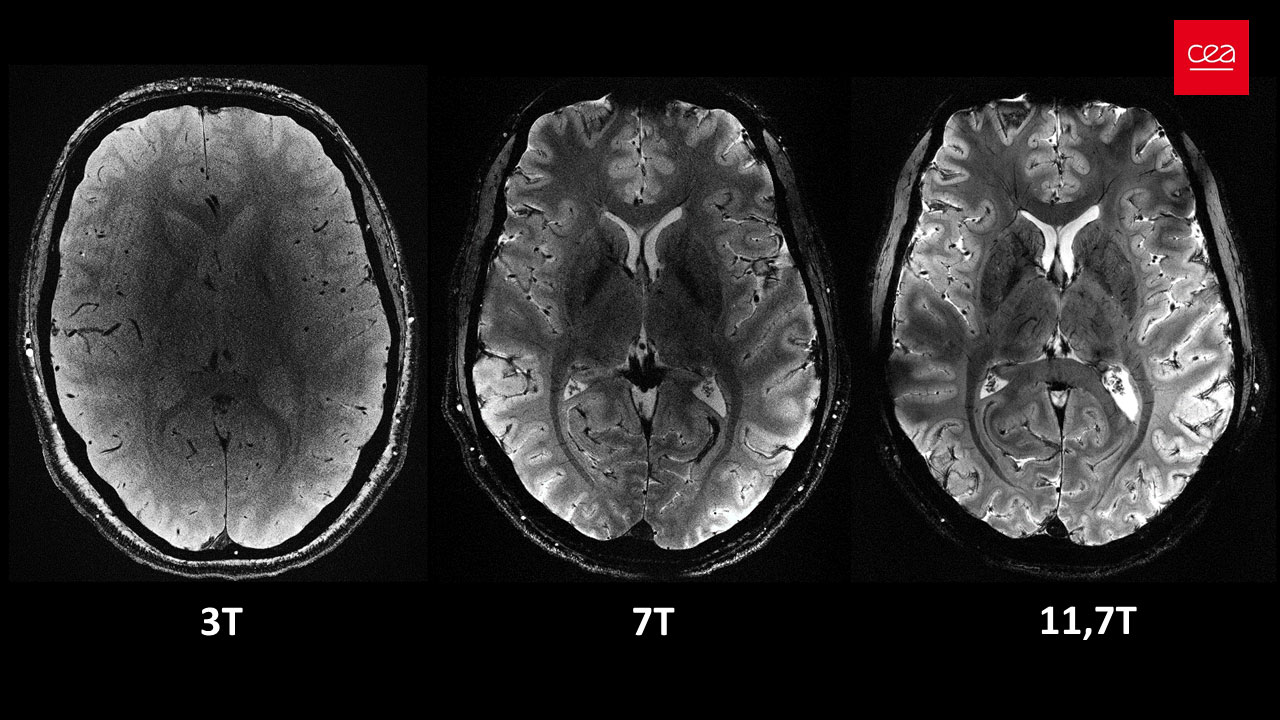
\includegraphics[width=\linewidth]{images/conclusion/cea-iseult.jpg}
\caption{\textbf{Axial sections of the human brain.} Most common MRI machines in hospitals have a magnetic field strength of 3 Tesla, producing brain images like the one on the far left. While only a few MRI machines worldwide reach 7 Tesla, the latest CEA Iseult MRI, with its unique 11.7 Tesla magnetic field, delivers exceptional results without any increase in exposure time.}
\label{fig:conclusion-ceaiseult}
\end{figure}


\noindent \textbf{VR/AR and LiDAR.} \ac{VR} and \ac{AR} have a long-standing history spanning 50 year. Recent advances in \ac{NeRF} have paved the way for \ac{VR}-oriented developments, such as VR-NeRF \citep{xu2023vr}, which enables real-time dual 2K generation in walkable virtual reality spaces. Apple's VisionPro mixed-reality headset, released in 2023 and marketed as a \textit{spatial computer}, is expected to have a major impact on how \ac{VR} and \ac{AR} are consumed on a daily basis by individuals. Associated operating system, termed \textit{visionOS}, will allow developers and researchers to to create 3D and \ac{CGI}-based applications on this new spatial computing platform.

LIDAR sensors are now integrated into nearly all flagship smartphones, opening up vast opportunities for research and development in highly detailed 3D reconstruction. The China-based startup \href{https://www.xgrids.com/}{XGRID} is working on a \ac{LiDAR}, multi-\ac{SLAM} and 3D\ac{GS}-based solution to build realistic large-scale 3D scenes, potentially at street or city level in the near future. These ultra-realistic scenes could then be processed using \ac{AI} and conventional graphics and game engines, such as Blender, Maya or UnrealEngine. 

\noindent \textbf{Animation and video games.} Finally, the animation and video games industries are about to undergo a significant revolution. Processes that have been in place for decades to animate 3D caracters or render highly detailed \ac{CGI} scenes are about to be disrupted by \ac{AI}. From storyboarding to 3D modeling and animation, creating a high-quality cartoon or animated film typically takes months or even years and involves dozens of skilled roles. \ac{AI} and 3D will streamline these costly production piplines. Recent advances in 3D meshes and 3D\ac{GS}-based rigging and animation \citep{qian2023gaussianavatars,li2024animatablegaussians} confirms that both animation and video production are set to  experience drastic changes in the near future. 

\ac{CGI}, widely used in the film industry, will also see major advancements thanks to the latest research in neural rendering and graphics. 3D\ac{GS}-based methods designed to address challenges in texture, shading and lightning have already been published \citep{jiang2023gaussianshader,wu2024deferredgs}, and the associated 3D scene can even be manually corrected and modified using \href{https://github.com/aras-p/UnityGaussianSplatting/}{Unity UnrealEngine add-on}. 


\section{IA challenges in 2024}

This section embrasses the most recent issues and trends currently shaping the 3D-related \ac{AI} landscape. It is not technical in nature but aims to cover the main challenges that the scientific community —from academic researchers to tech companies— and individuals will face in the months and years ahead.

\subsection{Open-source}
\label{sec:conclusion-open}
\ac{AI} has made its way into world with the release of ChatGPT by OpenAI in December 2022 of ChatGPT, a conversational chatbot based on \ac{LLM}. 

However, the underlying technology of \ac{LLM} was already well understood by scientific community years before its release. OpenAI was used to publish both code and technical notes on their latest advancements in their \textit{GPT} models. The GPT-2 model, a predecessor to ChatGPT, was notably permissive from a licencing perspective in 2018. However, this period of openness has since ended at OpenAI. The company now only releases source code for a few of its products, such as \textit{Whisper}, a general-purpose speech recognition model. The \ac{AI} community has witnessed a fundamental chisme in the way research and code are shared or kept secret. It puts back to back compagnies advocating for an open-source access to significant advancements in \ac{AI} against those arguing for the necessity to keep proprietary control over technologies and \ac{AI}-based algorithms that could be misused. MistralAI, HuggingFace, StabilityAI and even Meta now stand in opposition to companies like OpenAI, Anthropic, and MidJourney, chich market and distribute \ac{AI} products with technological foundations that remain inaccessible to academic researchers and individuals. 

I firmly believe that \ac{AI} research is now supported by a growing community of experts who are highly motivated by the forthcoming technological and intellectual challenges \ac{AI} is raising. Closed-proprietary \ac{AI} companies will ineluctably be overtaken by their open-source counterparts. Figure \ref{fig:conclusion-openclose} illustrates this claim for \ac{LLM}. 
\begin{figure}[htb!]
    \center
  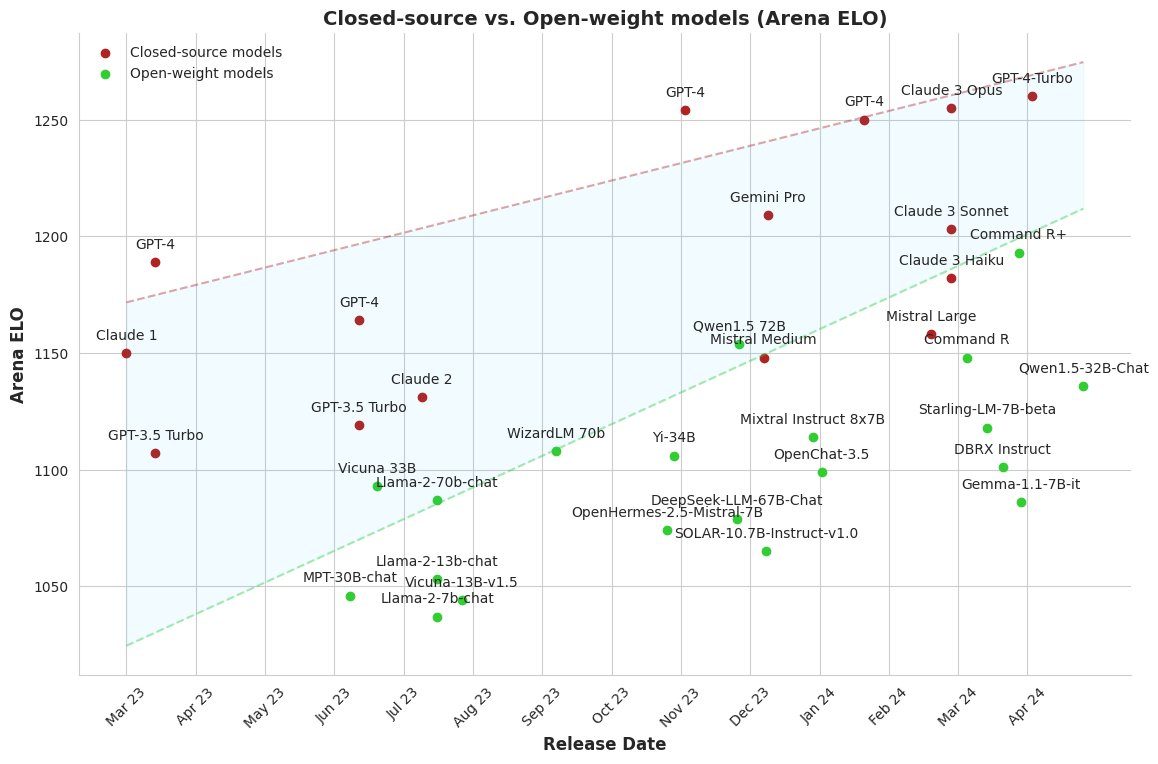
\includegraphics[width=\linewidth]{images/conclusion/open-close.jpeg}
  \caption{\textbf{LLMs ELO score based on human ratings.} Such graph is built on a regular monthly basis, thanks to \citep{chiang2024chatbot} work. It appears that open models now have a 6 to 10-month lag, compared to over a year when OpenAI's GPT-4 model was released.}
  \label{fig:conclusion-openclose}
\end{figure}


While 3D \ac{AI} is not as prominently affected by such a chisme as \ac{LLM}, we are currently observing an increasing number of startups raising funds to support one of the two models. StabilityAI, an already esteemed firm in the \ac{AI} landscape for its diffusion models \citep{esser2024scaling}, has recently made public a significant number of single-image 3D reconstruction models \citep{tochilkin2024triposr,voleti2024sv3d}. 

In the realm of 3D reconstruction and \ac{NVS} through 3D\ac{GS} considerations, the open-source framework \href{https://docs.gsplat.studio/main/}{gsplat} benefits from daily updates by the community. The code we are currently developing at CarCutter is also based on this commercially permissive library. 

\subsection{Fundation models and environmental issue}

Almost all modalities, from text (\textit{Mistral7B} by MistralAI, \textit{Llama2} by Meta, \textit{Claude3} by Antropic, and \textit{GPT-4} by OpenAI) to image (\textit{Stable Diffusion 3} by StabilityAI, \textit{DALL.E 3} by OpenAI, Midjourney \textit{V6}), as well as video (\textit{SoRA} by OpenAI, \textit{Gen-2} by Runway), now have their fundation models.The 3D domain, along with audio, may be among the last areas to not have reached this milestone \footnote{We exclude here the latest work in single-image 3D reconstruction, as it is still limited to centric object at low resolution.}. However, domains related to \ac{VR}, video games, or animation have not yet witnessed the \ac{AI} revolution that text and image have experienced in recent years. OpenAI CEO Sam Altman recently tweeted in April 2024 , affirming this shift: "movies are going to become video games and video games are going to become something unimaginably better". It is difficult not to recognize the growing importance that 3D will have in the coming years.

However, while an increasing numbers of models are now freely available, the \ac{GPU} ressources required to train or even perform inference with these models (which contain hundreds of millions to tens of billions of learnable parameters) remain substantial. One of the latest MistralAI model, called \textit{8x7B}, requires almost 700GB of vRAM \ac{GPU} for training (an 8-A100 \ac{GPU}s cluster would not be sufficient here) as shown on Table \ref{tab:gs-mistral_requirement}. 

\begin{table}[htp!]
  \caption{\textbf{ Mistral 8x7B model} Half and full precision vRAM GPU requirements for training. Figures from \href{https://huggingface.co/docs/accelerate/main/en/usage_guides/model_size_estimator}{HuggingFace Model Memory Calculator}}
  \label{tab:gs-mistral_requirement}
  \centering
  \begin{adjustbox}{width=\linewidth}
  \begin{tabular}[h]{c||cccc}
  \hline 
   Precision &  \textit{Model} & \textit{Gradient calculation} & \textit{Backward pass} & \textit{Optimizer step} \\
  \hline 
  \textbf{float16} \textit{(half)} & 174.4GB  & 261.7GB & 348.9GB & 348.9GB\\
  \textbf{float32} \textit{(full)} &  174.4GB  & 174.4GB & 348.9GB & 697.9GB \\
  \hline 
  \end{tabular}
  \end{adjustbox}
\end{table}
Factorial Funds estimates in one of its \href{https://www.factorialfunds.com/blog/under-the-hood-how-openai-s-sora-model-works}{report} that between $4.2K$ and $10K$ Nvidia H100 \ac{GPU}s are required for a whole month to train the latest text-to-video OpenAI \textit{SoRa} models. With a power consumption of 700W  per \ac{GPU}, the training of \textit{SoRA} has consummed as much as electricity in one month as a French individual does in 12 years. The same report also states that a single H100 can produce a 5-minute video in about an hour. If such innovative technology becomes publicly available in the coming months and years, Fcatorial Funds estimates that OpenAI will require approximately 720,000 H100 \ac{GPU} to meet global demand\footnote{Based on 50\% \ac{AI}-generated videos on TikTok for a daily basis and 15\% on Youtube.}. 

Finally, the current trend from NVDIA regarding its \ac{GPU} development is not geared toward energy efficiency. The primary goal is to continuously push toward higher FLOPS performance: while the next \ac{GPU} Blackwell generation, called B100 and B200, is expected to be 25 times faster than the H100, they will also have a power requirement of 1000W. 


\subsection{AI Ethics} 

Over the past five years, \ac{AI} has made significant progress at a stunning pace. As \ac{AI} capabalities strengthen every day, so does the need to tackle its associated ethical delemmas. 

Ethics is one of the main argument put forth by companies advocating for exclusive ownership of their \ac{AI} algorithms and products. They aim to ensure that such source codes remain out of the hands of those who might misuse them for malicious reasons. While \ac{AI}-based algorithms for audio or images were insufficiently developed a few years ago to deceive the human eye or ear, deck has been thoroughly reshuffled lately. However, \ac{AI} is not limited to generative content creation; decision-making granted by \ac{AI} are increasingly being adopted in various fields, including medical diagnostics for cancer detection (\eg Owkin) and  more controversial areas such as military applications (\eg Anduril).

In March 2024, OpenAI introduced one of its latest products, the \href{https://openai.com/blog/navigating-the-challenges-and-opportunities-of-synthetic-voices}{Voice Engine}. A 15-second audio recording is now sufficient to clone a human voice with remarkable accuracy using this \ac{AI}. While OpenAI emphasizes the positive potentials offered by their technology (such as for live translation or assisting individuals with oral disorders), the company also conceeds that its product brings significant threats, including telephone fraud or identity theft. 

The first deepfakes, which emerged in 2017, referred specifically to videos in which a person's face was artificially altered by \ac{AI} to assume the appearance of someone else. Since then, the definition has broadened considerably. In April 2024, Microsoft released a technology called VASA-1 \citep{xu2024vasa1}, which enables the generation of voiced deepfakes from a single image. Similar to OpenAI, Microsoft has already communicated the potential threats and misuses that VASA-1 could entail, although no public release has been announced yet.

In mid-2023, Google developed SynthID, a tool that enables for watermarking \ac{AI}-generated image and audio. This indirectly helps to protect original human content creation. Decision-making political authorities and parliaments worldwide are beggining to urge their partners to regulate \ac{AI} and establish a coherent legal framework. The AI Act was ratified in Europe in February 2024 and is set to take effect in 2025. It will impose a certain transparency requirements regarding the training data used for foundation models and biais studies related to the outcomes produced by such \ac{AI} models. As of now, the US government does not have such a similiar AI Act. 


